\documentclass[aspectratio=169]{beamer}

% ── Theme ────────────────────────────────────────────────────────────────────
\usetheme{Madrid}
\usecolortheme{default}
\setbeamertemplate{navigation symbols}{}
\setbeamertemplate{footline}[frame number]

% ── Packages ─────────────────────────────────────────────────────────────────
\usepackage{booktabs}
\usepackage{microtype}
\usepackage{xcolor}
\usepackage{listings}
\usepackage{tikz}
\usetikzlibrary{arrows.meta, positioning, shapes.geometric, fit, backgrounds}
\usepackage{fontawesome5}
\usepackage{multirow}
\usepackage{array}
\usepackage{graphicx}

% ── Colours ──────────────────────────────────────────────────────────────────
\definecolor{symptom}    {HTML}{E57373}   % red
\definecolor{condition}  {HTML}{64B5F6}   % blue
\definecolor{testcol}    {HTML}{81C784}   % green
\definecolor{vital}      {HTML}{FFB74D}   % orange
\definecolor{demo}       {HTML}{CE93D8}   % purple
\definecolor{riskfactor} {HTML}{FFF176}   % yellow
\definecolor{moi}        {HTML}{F48FB1}   % rose
\definecolor{attribute}  {HTML}{80CBC4}   % mint
\definecolor{treatment}  {HTML}{A5D6A7}   % light green
\definecolor{adverseev}  {HTML}{FFCCBC}   % peach

\definecolor{darkblue}   {HTML}{1A237E}
\definecolor{midblue}    {HTML}{1565C0}
\definecolor{lightgray}  {HTML}{F5F5F5}

\setbeamercolor{frametitle}      {bg=darkblue, fg=white}
\setbeamercolor{title}           {fg=white}
\setbeamercolor{palette primary} {bg=darkblue, fg=white}
\setbeamercolor{palette secondary}{bg=midblue,  fg=white}
\setbeamercolor{structure}       {fg=darkblue}

% ── Listing style ─────────────────────────────────────────────────────────────
\lstset{
  basicstyle=\ttfamily\footnotesize,
  backgroundcolor=\color{lightgray},
  frame=single,
  rulecolor=\color{gray!40},
  breaklines=true,
  columns=fullflexible,
  keepspaces=true,
}

% ── Helper commands ───────────────────────────────────────────────────────────
\newcommand{\nodebox}[2]{%
  \colorbox{#1}{\strut\small\textbf{#2}}%
}

% ── Metadata ─────────────────────────────────────────────────────────────────
\title[Medical Triage KG]{Medical Triage Knowledge Graph}
\subtitle{A Multi-Ontology GraphRAG Pipeline for Emergency Department Decision Support}
\author{LMP2392 --- Healthcare and Medicine for AI Experts}
\date{\today}

% ─────────────────────────────────────────────────────────────────────────────
\begin{document}
% ─────────────────────────────────────────────────────────────────────────────

% ── Title slide ───────────────────────────────────────────────────────────────
\begin{frame}
  \titlepage
\end{frame}

% ── Outline ───────────────────────────────────────────────────────────────────
\begin{frame}{Outline}
  \tableofcontents
\end{frame}

% =============================================================================
\section{System Architecture}
% =============================================================================

\begin{frame}{High-Level Architecture}
  \centering
  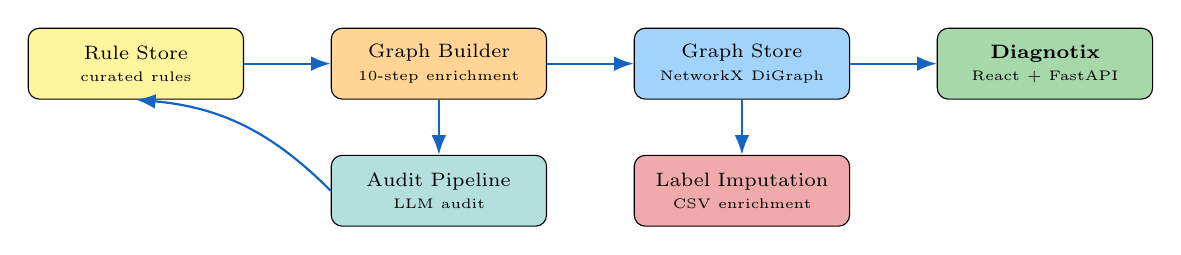
\begin{tikzpicture}[
    node distance=0.7cm and 1.1cm,
    box/.style={draw, rounded corners, fill=lightgray,
                text width=2.5cm, align=center, minimum height=0.9cm,
                font=\scriptsize},
    arr/.style={-{Latex[length=2.5mm]}, thick, color=midblue},
  ]
    \node[box, fill=riskfactor!70] (json)
      {Rule Store\\{\tiny curated rules}};

    \node[box, fill=vital!60, right=of json] (build)
      {Graph Builder\\{\tiny 10-step enrichment}};

    \node[box, fill=condition!60, right=of build] (pkl)
      {Graph Store\\{\tiny NetworkX DiGraph}};

    \node[box, fill=testcol!70, right=of pkl] (diagnotix)
      {\textbf{Diagnotix}\\{\tiny React + FastAPI}};

    \node[box, fill=symptom!60, below=of pkl] (pipe)
      {Label Imputation\\{\tiny CSV enrichment}};

    \node[box, fill=attribute!60, below=of build] (audit)
      {Audit Pipeline\\{\tiny LLM audit}};

    \draw[arr] (json)         -- (build);
    \draw[arr] (build)        -- (pkl);
    \draw[arr] (pkl)          -- (diagnotix);
    \draw[arr] (pkl)          -- (pipe);
    \draw[arr] (build.south)  -- (audit.north);
    \draw[arr] (audit.west)   to[bend right=20] (json.south);
  \end{tikzpicture}

  \vspace{0.4em}
  \small
  Rules are iteratively audited and revised until satisfactory, then
  the graph builder serialises the final graph. The graph store
  powers \textbf{Diagnotix} for dynamic expansion and
  label imputation for CSV enrichment.
\end{frame}

% =============================================================================
\section{Knowledge Graph Construction}
% =============================================================================

\begin{frame}{10-Step Enrichment Pipeline (Graph Builder)}
  \scriptsize
  \begin{tabular}{@{}clll@{}}
    \toprule
    \textbf{Step} & \textbf{API / Source} & \textbf{Enriches} & \textbf{Column(s) added} \\
    \midrule
    0 & Static rules          & ---               & base DataFrame \\
    1 & URL Registry                  & \texttt{(source, test)} & \texttt{url} \\
    2 & EMBL-EBI OLS4 (HP/MONDO/EFO) & \texttt{raw\_symptom} & \texttt{ebi\_code}, \texttt{synonyms} \\
    3 & Infoway FHIR (SNOMED CT CA)  & \texttt{raw\_symptom} & \texttt{infoway\_code} \\
    4 & UMLS REST (LOINC)            & \texttt{test}         & \texttt{loinc\_code} \\
    5 & UMLS REST (ICD-10 international) & \texttt{condition} & \texttt{icd10\_code} \\
    6 & Infoway FHIR (ICD-10-CA)     & \texttt{condition}    & \texttt{icd10ca\_code} \\
    7 & NLM RxNorm + OpenFDA         & \texttt{treatment}    & \texttt{rxcui}, \texttt{adverse\_event} \\
    8 & Europe PMC                   & symptom \(\leftrightarrow\) condition & \texttt{literature\_weight} \\
    9 & Europe PMC                   & condition \(\leftrightarrow\) test & \texttt{test\_literature\_weight} \\
    10 & ClinicalTrials.gov v2       & condition \(\leftrightarrow\) treatment & \texttt{trial\_count} \\
    \bottomrule
  \end{tabular}

  \vspace{0.4em}
  Steps 8--10 attach \textbf{real-world evidence counts} that drive edge-width
  scaling in the HTML visualisation.
\end{frame}

% =============================================================================
\section{Guideline Audit Pipeline}
% =============================================================================

\begin{frame}{Audit Pipeline Overview}
  \textbf{Problem:} LLM-generated rules can be fabricated, vague, or misattributed.
  The audit pipeline cleans the rule store before the graph is built.

  \vspace{0.5em}
  \centering
  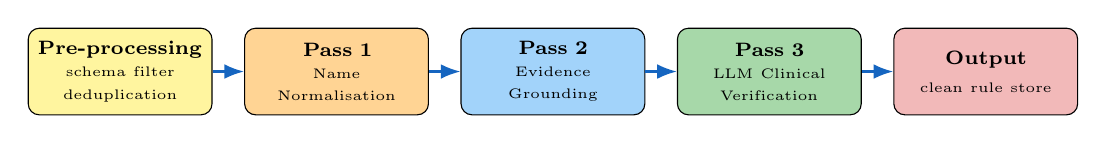
\begin{tikzpicture}[
    node distance=0.4cm and 0.4cm,
    box/.style={draw, rounded corners, fill=lightgray,
                text width=2.1cm, align=center, minimum height=1.1cm,
                font=\scriptsize},
    arr/.style={-{Latex[length=2.5mm]}, thick, color=midblue},
  ]
    \node[box, fill=riskfactor!70] (pre)
      {\textbf{Pre-processing}\\[2pt]{\tiny schema filter\\deduplication}};
    \node[box, fill=vital!60, right=of pre] (norm)
      {\textbf{Pass 1}\\[2pt]{\tiny Name\\Normalisation}};
    \node[box, fill=condition!60, right=of norm] (ground)
      {\textbf{Pass 2}\\[2pt]{\tiny Evidence\\Grounding}};
    \node[box, fill=testcol!70, right=of ground] (verify)
      {\textbf{Pass 3}\\[2pt]{\tiny LLM Clinical\\Verification}};
    \node[box, fill=symptom!50, right=of verify] (out)
      {\textbf{Output}\\[2pt]{\tiny clean rule store}};

    \draw[arr] (pre)    -- (norm);
    \draw[arr] (norm)   -- (ground);
    \draw[arr] (ground) -- (verify);
    \draw[arr] (verify) -- (out);
  \end{tikzpicture}

  \vspace{0.3em}
  \begin{columns}[T]
    \begin{column}{0.24\textwidth}
      \footnotesize
      \textbf{Pre-processing}\\
      Drop rules with missing fields or unknown sources.
      Remove exact duplicate triples from repeated generation passes.
    \end{column}
    \begin{column}{0.24\textwidth}
      \footnotesize
      \textbf{Pass 1 — Normalise}\\
      Replace LLM-invented names with canonical labels \emph{before} LLM review:
      ICD-10 international (UMLS) and HP/MONDO (OLS4).
    \end{column}
    \begin{column}{0.24\textwidth}
      \footnotesize
      \textbf{Pass 2 — Ground}\\
      Fetch Europe PMC article counts + DuckDuckGo snippets.
      Tag each rule with a PMC evidence tier.
    \end{column}
    \begin{column}{0.24\textwidth}
      \footnotesize
      \textbf{Pass 3 — Verify}\\
      LLM reviews each pathway in batches of $\leq$15.
      Evidence tier sets the retention bias.
    \end{column}
  \end{columns}
\end{frame}

% =============================================================================
\section{Diagnotix Web Application}
% =============================================================================

\begin{frame}{Diagnotix --- Interactive Knowledge Graph Explorer}
  \centering
  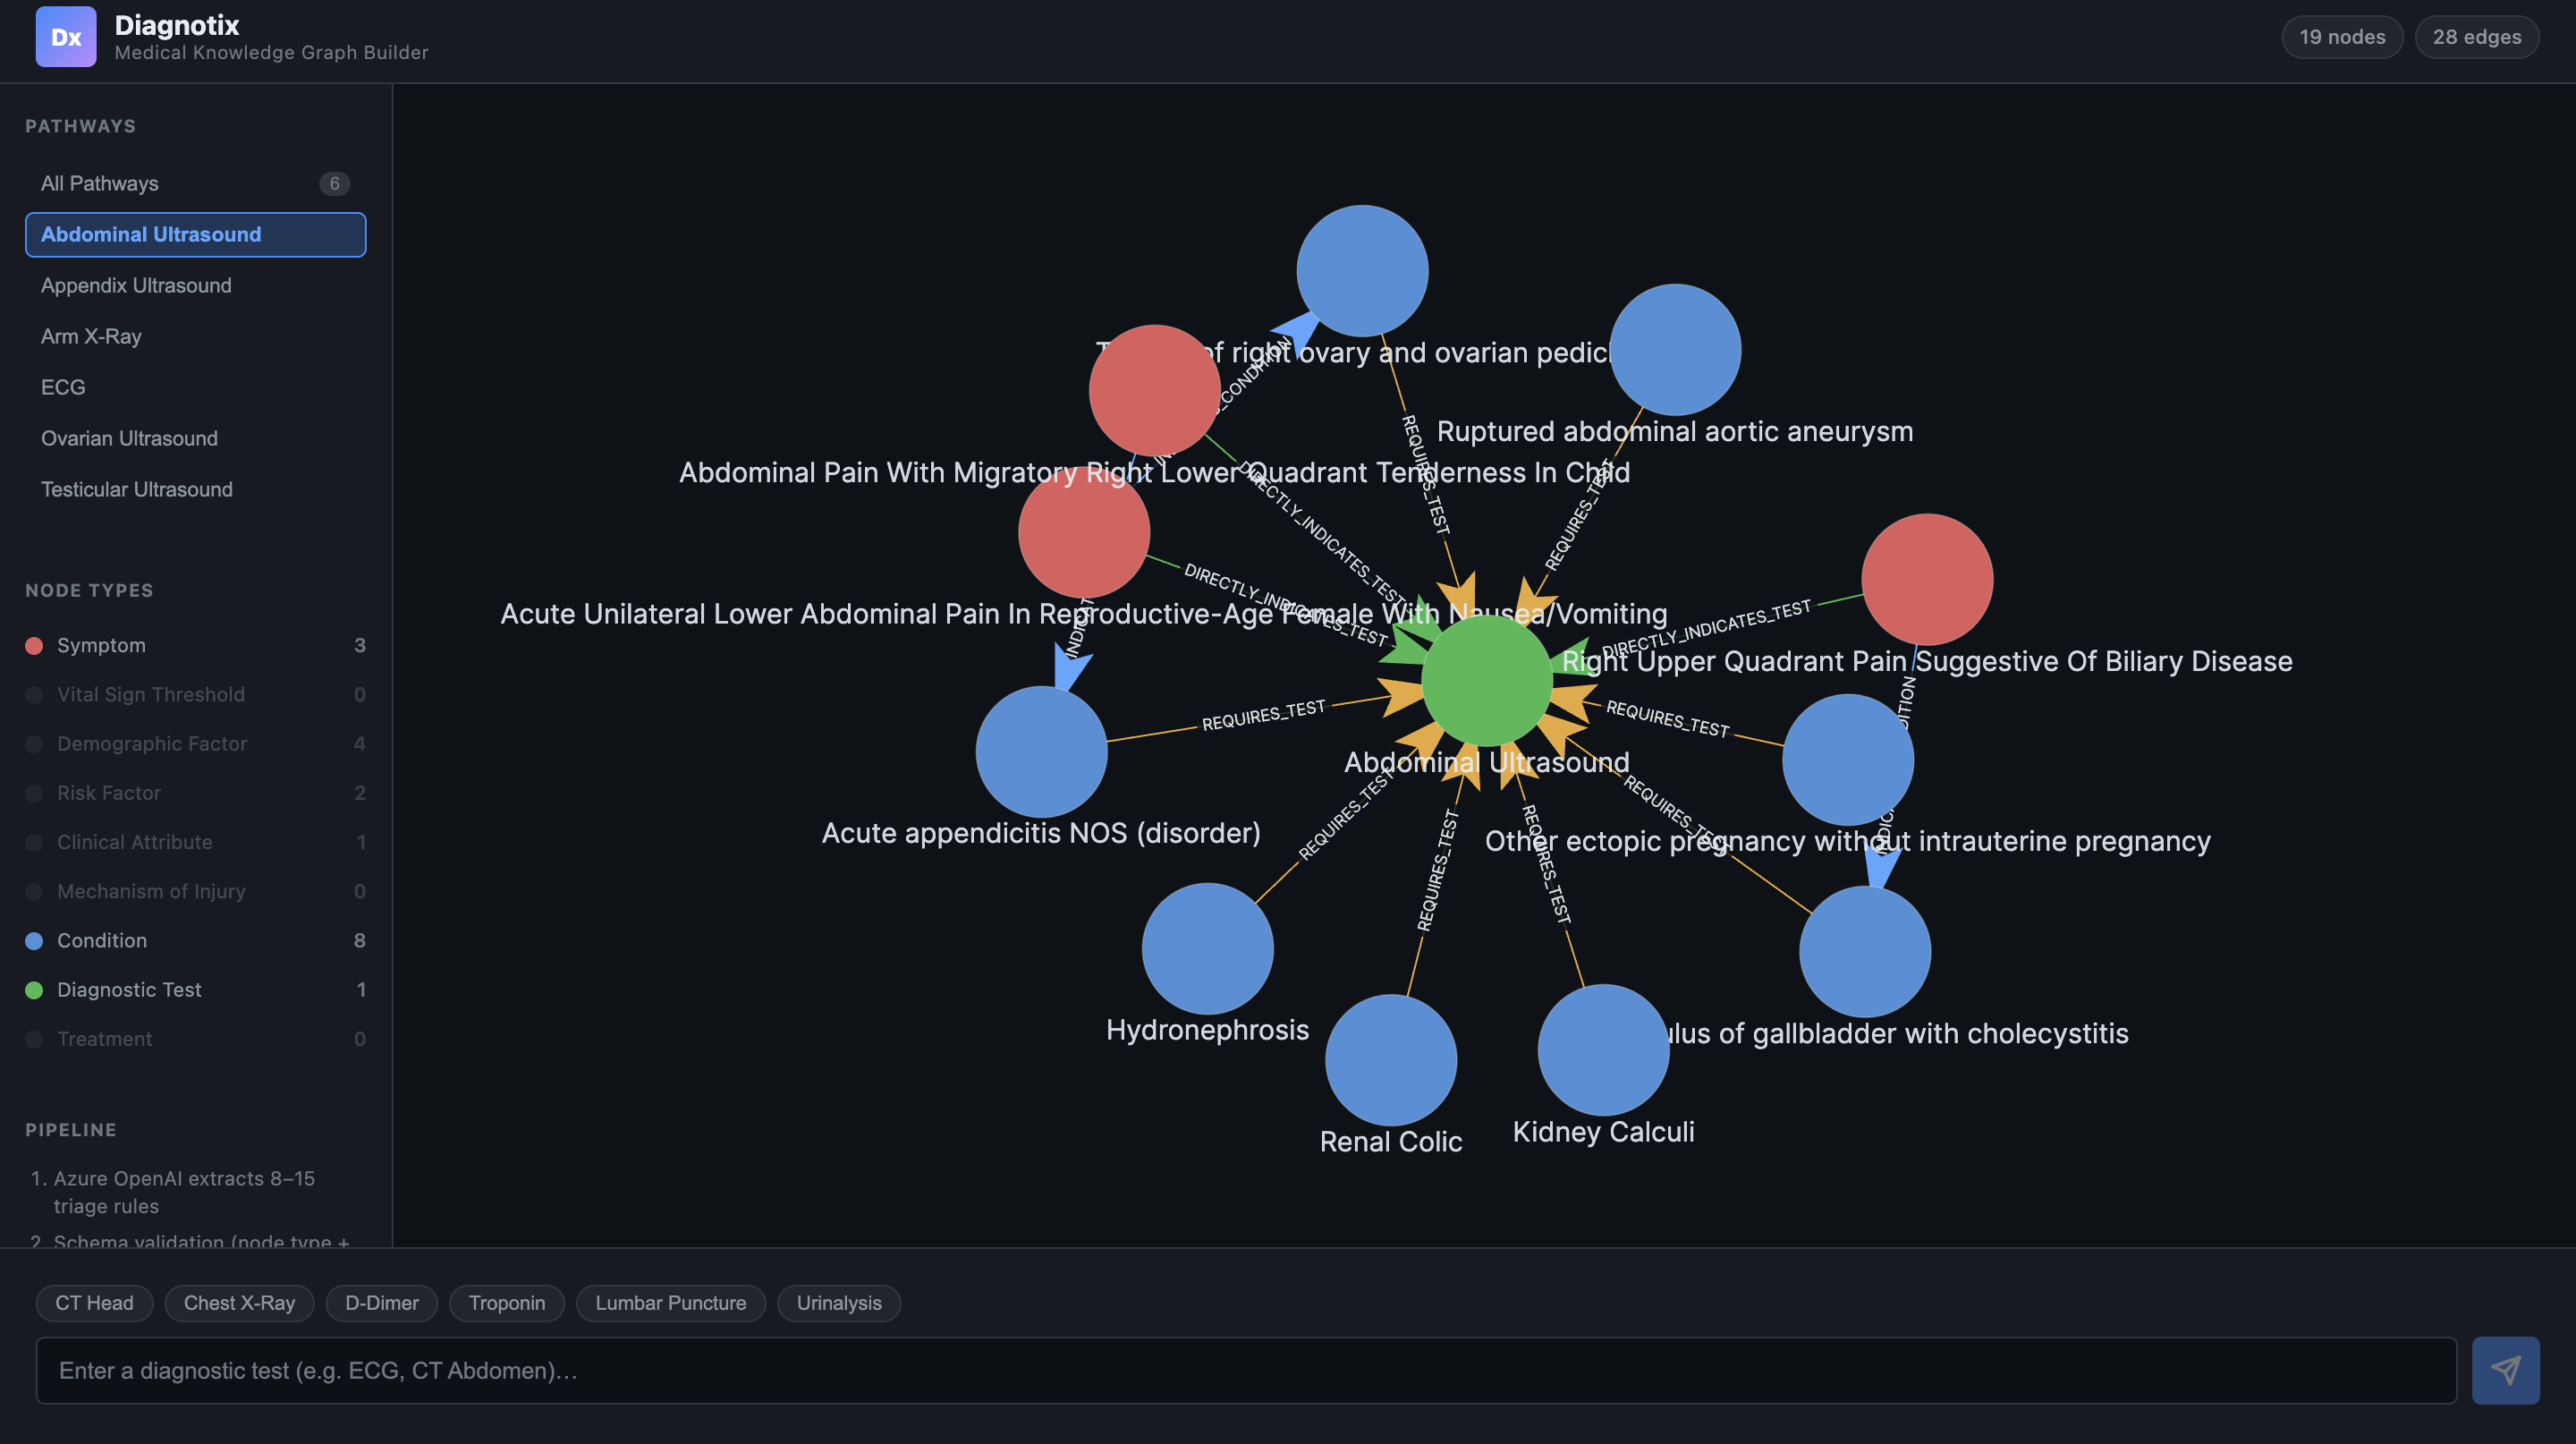
\includegraphics[width=0.95\linewidth]{images/webapp-ss.png}
\end{frame}

% =============================================================================
\section{Summary}
% =============================================================================

\begin{frame}{Summary}
  \small
  \begin{columns}[T]
    \begin{column}{0.48\textwidth}
      \textbf{What we built}
      \begin{itemize}
        \item An expandable knowledge graph spanning 5 clinical
              pathways, grounded in evidence-based guidelines.
        \item 10-step ontology enrichment pipeline (SNOMED CT CA,
              LOINC, ICD-10 international, ICD-10-CA, HP/MONDO,
              RxNorm, Europe PMC, ClinicalTrials.gov).
        \item Evidence-grounded audit pipeline: Europe PMC +
              web search evidence tiers inform LLM verification
              to reduce hallucinated rule retention.
        \item Two-phase data processing pipeline for back-mapping
              patient diagnoses to recommended diagnostic tests.
      \end{itemize}
    \end{column}
    \begin{column}{0.48\textwidth}
      \textbf{Future work}
      \begin{itemize}
        \item Continuously improve the audit pipeline to maintain
              knowledge graph accuracy over time.
        \item Integration with the SickKids database
              (where feasible).
        \item Extend from \emph{back prediction} (diagnosis
              $\to$ test) to \emph{front prediction} --- using
              patient vitals at triage to recommend tests,
              grounded in the knowledge graph.
        \item Expert clinician verification of the constructed
              knowledge graph.
      \end{itemize}
    \end{column}
  \end{columns}
\end{frame}

% =============================================================================
% APPENDIX — Additional slides
% =============================================================================
\appendix

\begin{frame}
  \centering
  \vspace{2em}
  {\Large\textbf{Additional Slides}}
\end{frame}

% ── Motivation ────────────────────────────────────────────────────────────────
\begin{frame}{The Clinical Problem}
  \begin{columns}[T]
    \begin{column}{0.55\textwidth}
      \textbf{Emergency Department triage is time-critical}
      \begin{itemize}
        \item Clinicians must rapidly map presenting symptoms to the right
              diagnostic test under cognitive and time pressure.
        \item Clinical guidelines (AHA/ACC, ACR, NICE, CTAS) encode
              evidence-based rules --- but they are dispersed across
              long PDFs and multiple organisations.
        \item LLMs alone can \emph{hallucinate} clinical pathways; they
              lack grounded, citable reasoning.
      \end{itemize}
      \vspace{0.5em}
      \textbf{Our answer: a knowledge graph as the ground truth layer.}
    \end{column}
    \begin{column}{0.42\textwidth}
      \begin{block}{Target pathways}
        \begin{tabular}{ll}
          \faHeartbeat    & ECG \\
          \faSearch       & Testicular Ultrasound \\
          \faBone         & Arm X-Ray \\
          \faNotesMedical & Abdominal Ultrasound \\
          \faNotesMedical & Appendix Area Ultrasound \\
        \end{tabular}
      \end{block}
      \begin{block}{Guideline sources}
        \small AHA/ACC \quad ACR \quad NICE \quad CTAS
      \end{block}
    \end{column}
  \end{columns}
\end{frame}

% ── Knowledge Graph Construction ──────────────────────────────────────────────
\begin{frame}[fragile]{Source of Truth: The Clinical Rule Store}
  Each of the 45 rules encodes a single clinical assertion:

  \vspace{0.3em}
  \begin{center}
    \texttt{raw\_symptom} \;\(\longrightarrow\)\; \texttt{condition} \;\(\longrightarrow\)\; \texttt{test}
  \end{center}

  \vspace{0.3em}
  \begin{columns}[T]
    \begin{column}{0.48\textwidth}
      \begin{exampleblock}{Example rule (JSON)}
        \begin{lstlisting}[language={}]
{
  "raw_symptom": "chest pain",
  "node_type": "Symptom",
  "condition": "Acute MI",
  "test": "ECG",
  "source": "AHA/ACC"
}
        \end{lstlisting}
      \end{exampleblock}
    \end{column}
    \begin{column}{0.48\textwidth}
      \begin{block}{Rule fields}
        \small
        \begin{tabular}{@{}ll@{}}
          \textbf{Field}      & \textbf{Meaning} \\
          \midrule
          \texttt{raw\_symptom} & Clinical entity \\
          \texttt{node\_type}   & KG category \\
          \texttt{condition}    & Target diagnosis \\
          \texttt{test}         & Recommended test \\
          \texttt{source}       & Guideline body \\
        \end{tabular}
      \end{block}
    \end{column}
  \end{columns}
\end{frame}

\begin{frame}{Graph Schema}
  \begin{columns}[T]
    \begin{column}{0.44\textwidth}
      \textbf{Primary node types}\\[0.4em]
      \begin{tabular}{@{}ll@{}}
        \nodebox{symptom!80}{Symptom}     & \texttt{Symptom:} \\[2pt]
        \nodebox{condition!80}{Condition} & \texttt{Condition:} \\[2pt]
        \nodebox{testcol!80}{Test}        & \texttt{Test:} \\
      \end{tabular}

      \vspace{0.6em}
      \textbf{Secondary node types}\\[0.4em]
      \begin{tabular}{@{}ll@{}}
        \nodebox{vital!80}{Vital}            & \texttt{Vital:} \\[2pt]
        \nodebox{demo!70}{Demographic}       & \texttt{Demographic:} \\[2pt]
        \nodebox{riskfactor!80}{Risk Factor} & \texttt{Risk Factor:} \\[2pt]
        \nodebox{moi!70}{MOI}                & \texttt{MOI:} \\[2pt]
        \nodebox{attribute!80}{Attribute}    & \texttt{Attribute:} \\[2pt]
        \nodebox{treatment!80}{Treatment}    & \texttt{Treatment:} \\
      \end{tabular}
    \end{column}
    \begin{column}{0.53\textwidth}
      \textbf{Edge types}\\[0.4em]
      \begin{tabular}{@{}ll@{}}
        \texttt{INDICATES\_CONDITION}     & entity \(\to\) condition \\[2pt]
        \texttt{REQUIRES\_TEST}           & condition \(\to\) test \\[2pt]
        \texttt{DIRECTLY\_INDICATES\_TEST}& entity \(\to\) test \\[2pt]
        \texttt{RECOMMENDS\_TREATMENT}    & condition \(\to\) drug \\
      \end{tabular}

      \vspace{0.8em}
      \textbf{Edge metadata on every edge:}
      \begin{itemize}
        \item \texttt{source} --- guideline body (AHA/ACC, ACR, \ldots)
        \item \texttt{source\_url} --- citable DOI or page URL
        \item evidence weight (literature / trial count)
      \end{itemize}
    \end{column}
  \end{columns}
\end{frame}

% ── Guideline Audit Pipeline ──────────────────────────────────────────────────
\begin{frame}{Audit Pipeline --- Evidence Grounding \& Verification}
  \begin{columns}[T]
    \begin{column}{0.48\textwidth}
      \begin{block}{Pass 2 --- Evidence Grounding}
        \small
        Two signals fetched per rule:
        \begin{itemize}
          \item \textbf{Europe PMC} co-occurrence count
          \item \textbf{DuckDuckGo} web snippets
        \end{itemize}
        \vspace{0.2em}
        Rules tagged by \textbf{PMC evidence tier}:
        \begin{center}
          \footnotesize
          \begin{tabular}{@{}ll@{}}
            \textbf{STRONG}   & $\geq$5\,000 articles \\
            \textbf{GOOD}     & $\geq$500 \\
            \textbf{MODERATE} & $\geq$50 \\
            \textbf{LIMITED}  & $>$0 \\
            \textbf{NONE}     & 0 \\
          \end{tabular}
        \end{center}
        Zero-evidence rules flagged for clinician review.
      \end{block}
    \end{column}
    \begin{column}{0.48\textwidth}
      \begin{block}{Pass 3 --- LLM Clinical Verification}
        \small
        LLM reviewer grouped by pathway, batched at \textbf{$\leq$15 rules/call}.

        \vspace{0.2em}
        Evidence tier drives retention bias:
        \begin{itemize}
          \item STRONG / GOOD $\to$ retain by default
          \item MODERATE / LIMITED $\to$ normal scrutiny
          \item NONE $\to$ bias to remove
        \end{itemize}

        \vspace{0.2em}
        Three verification criteria:
        \begin{enumerate}
          \item Source accuracy
          \item Clinical plausibility
          \item Condition specificity
        \end{enumerate}
      \end{block}
    \end{column}
  \end{columns}
\end{frame}

% ── Data Processing Pipeline ──────────────────────────────────────────────────
\begin{frame}{Data Processing Pipeline --- Two-Phase Overview}
  \textbf{Goal:} ingest a real patient CSV and enrich every diagnosis with
  KG-derived diagnostic tests.

  \vspace{0.5em}
  \begin{columns}[T]
    \begin{column}{0.48\textwidth}
      \begin{block}{Phase 1 --- Extract candidate tests}
        \textbf{Test Extractor}\\[0.3em]
        Reads all unique diagnoses from the \texttt{dx} column and asks
        GPT-5 Nano to identify the standard diagnostic test(s) for each.
        Writes a diagnosis-to-test mapping file.
      \end{block}
    \end{column}
    \begin{column}{0.48\textwidth}
      \begin{block}{Phase 2 --- Expand graph \& map patients}
        \textbf{Enrichment \& Mapping Pipeline}\\[0.3em]
        Adds any new test pathways to the KG, rebuilds the graph with full
        ontology enrichment, then maps every diagnosis back to a condition
        node and its recommended tests.
      \end{block}
    \end{column}
  \end{columns}

  \vspace{0.5em}
  \begin{block}{Standalone mapping (graph already current)}
    \textbf{Label Imputation} --- skips graph expansion; semantically maps a
    new patient CSV against the existing graph store via GPT-5 Nano.
  \end{block}
\end{frame}

% ── Diagnotix Web Application ─────────────────────────────────────────────────
\begin{frame}[fragile]{Diagnotix --- Dynamic Knowledge Graph Builder}
  \begin{columns}[T]
    \begin{column}{0.52\textwidth}
      \textbf{Full-stack web application (FastAPI + React)}

      \begin{itemize}
        \item Enter any diagnostic test name; the LLM extracts
              8--15 evidence-based triage rules automatically.
        \item Generated rules are validated via an evidence-grounded
              audit pipeline: Europe PMC co-occurrence + DuckDuckGo
              web search ground each rule before LLM clinical review.
        \item Validated rules are appended to the rule store and the
              full ontology enrichment pipeline re-runs.
        \item Every expansion is auditable: the response reports
              new rule count and updated node/edge totals.
      \end{itemize}
    \end{column}
    \begin{column}{0.45\textwidth}
      \begin{block}{Stack}
        \small
        Backend: FastAPI + Uvicorn\\
        Frontend: React 19 + TypeScript + Vite\\
        LLM: GPT-5 Nano
      \end{block}
      \begin{block}{Node tooltip codes}
        \small
        \begin{tabular}{@{}ll@{}}
          HP/MONDO    & SNOMED-CT \\
          ICD-10$^{*}$ (linked) & ICD-10-CA \\
          LOINC       & RxCUI \\
        \end{tabular}\\[2pt]
        \tiny $^{*}$links to WHO ICD-10 browser
      \end{block}
    \end{column}
  \end{columns}
\end{frame}

% ─────────────────────────────────────────────────────────────────────────────
\end{document}
